\label{referencial}

Neste Capítulo apresentamos a primeira etapa do \textit{Design Science Research} -- Compreensão do problema -- onde apresentamos os conceitos necessários para o entendimento deste trabalho, passando pelos pontos da Engenharia de Software, Engenharia de Requisitos, elicitação de requisitos, Desenvolvimento Ágil de Software, Metodologia Scrum, \textit{Planning Poker}, Inteligência Artificial, Ética em \acrshort{IA}, Agentes morais versus sistemas baseados em IA em conformidade com princípios éticos e os trabalhos relacionados, qual será o nosso esforço de pesquisa.

\section{Engenharia de Software}

 A partir do início da década de 1940, os computadores eram criados com um fim específico, rodando apenas para o fim específico ao qual foi projetado, como por exemplo o Colossus, primeira máquina computacional criada  por Alan Turing que se tem registrado, com o fim de decifrar mensagens criptografadas enviadas pelos alemães \cite{colossus}. Esta era uma época onde máquinas eram construídas para realizar apenas um único propósito computacional programável, com uma única tarefa a ser executada desde o princípio de sua existência. Pouco tempo após, vimos a criação dos primeiros computadores que permitiam rodar mais do que um único programa, lendo a partir de cartões perfurados o que o computador deveria executar ou qual poderia ser uma resposta esperada, conforme descrito por Dijsktra \cite{Humble}. 
 
 Com o passar do tempo, miniaturização, modernização e a popularização dos computadores, podendo estes serem usados dentro de firmas empresariais, órgãos governamentais, universidades e até mesmo em casas (apesar dos proibitivos preços), fazendo assim com que novas gamas de capacidades fossem dadas aos computadores. Com isto, naturalmente novos softwares e linguagens de programação foram sendo criados, e trazendo consigo o início da popularização das áreas de desenvolvimento de software e como estas poderiam produzir um produto de qualidade com um tempo razoável e um custo factível. Porém, o que se viam era exatamente o contrário, onde durante a produção destes aplicativos víamos projetos estourando o orçamento e o tempo previsto, uma qualidade bem aquém do esperado, não atendiam ao usuário final devidamente e de custosa manutenção e verificação dos códigos, conforme foi constado por Naur e Randell na conferência do comitê de ciência da Organização do Tratado do Atlântico Norte (\acrshort{OTAN}) \cite{NATO}. A partir daí, verificando que alguns métodos derivados da administração poderiam funcionar também na produção de software, vemos o nascimento de métodos formais para o auxílio na construção de tais ferramentas de uso computacional. E daí, temos a criação do desenvolvimento da área de Engenharia de software, também citada pela primeira vez na conferência do comitê de ciência da \acrshort{OTAN} \cite{NATO}. 

Engenharia de software é o processo que foca nas áreas de planejamento, desenvolvimento e entrega dos sistemas de software. É com este tipo de metodologia que conseguimos estimar de maneira mais apurada formas de como desenvolver o sistema, estimar prazos, recursos e até mesmo espaços para melhora durante e após a conclusão do projeto. A engenharia de software nasceu da necessidade de entregar ao cliente uma maior garantia de qualidade, sem deixar de lado a preocupação com prazos, estes cada vez mais curtos perante as demandas que o mundo e sua evolução tecnológica tem exigido de acordo Sommerville\cite{Sommerville07}. Para Pressman \cite{pressman}, a Engenharia de Software envolve processos, métodos e ferramentas que permitem aos profissionais
construir softwares bem desenvolvidos. Para Wazlawick \cite{wazlawick}, a Engenharia de Software é olhada como o meio de estudo, criação e otimização de processos para o desenvolvimento de software, onde as atividades essenciais de um engenheiro de software envolve a especificação do software, seu desenvolvimento, validação e sua evolução.

Uma dos motivos que a Engenharia de Software se tornou algo extremamente relevante é a crescente necessidade da sociedade e dos indivíduos e como se relacionam com os sistemas de software, onde estes necessitam ser pensados e projetados com a maior excelência possível para se ter segurança, performance e possibilidade de manutenção. A partir de um olhar no aspecto econômico, um outro motivo é que, a longo prazo, se torna mais barato utilizar técnicas e métodos de Engenharia de Software ao invés de projetar sistemas sem a padronização demandada sem estas técnicas e métodos, já que para a maior parte dos de sistemas de software, boa parte dos custos estão ligados as modificações realizadas no software após sua implantação, quando este já se encontra em produção \cite{Sommerville07}.

Em suma, a Engenharia de Software é uma disciplina que envolve diversas áreas, à exemplo: processos de software, desenvolvimento ágil, engenharia de requisitos, testes
de software, evolução de software e segurança. Assim, se dá a importância crucial dos sistemas de software para todos os aspectos da nossa sociedade atual.

\subsection{Engenharia de Requisitos}

A engenharia de requisitos (ou especificação de software) é a área responsável por entender e decidir quais serão as requisições necessárias ao sistema solicitado e verificar os impedimentos relacionados ao desenvolvimento e operação do sistema. Costuma ser um estágio crítico do processo de criação de um software, pois uma vez mal desenhado e com erros nesta fase, mais a frente no projeto, implantação e manutenção do sistema problemas serão comuns de aparecerem, segundo Sommerville \cite{Sommerville07}. Para Pressman \cite{pressman}, é a área que engloba as tarefas e técnicas que guiam a uma noção mais precisa possível dos requisitos, sendo esta uma das ações principais da Engenharia de Software. 
Esta etapa existe com o propósito de criar uma documentação de requisitos acordados onde cria a especificação de um sistema que possa atender às necessidades dos clientes atendidos para o desenvolvimento do software. Usualmente, os requisitos são postos para seus clientes e usuários finais em um nível mais alto, sem grandes detalhes técnicos, enquanto para os desenvolvedores é essencial que os detalhes técnicos sejam muito bem apresentados \cite{Sommerville07}.

De acordo Sommerville \cite{Sommerville07}, são quatro níveis principais do processo de engenharia de requisitos, conforme apresentado na Figura \ref{fig:eng_req}, os quais são:

\begin{enumerate}
    \item \textbf{Estudo de viabilidade}: Realiza-se uma aproximação a respeito a possibilidade de se cumprir com as requisições do usuário em questão, valendo-se de tecnologias contemporâneas, seja a nível de software ou de hardware. Esse estudo leva em conta se o sistema a ser criado será lucrativo sobre uma posição de negócio e se o mesmo pode ser construído sob condições financeiras limitadas. Um estudo de viabilidade deve ser algo sem grandes custos e de rápida conclusão, onde o resultado culmina na decisão ou não de continuar com a possibilidade de um estudo mais detalhado.
    
    \item \textbf{Elicitação e análise de requisitos}: Esta é a parte do processo onde se inicia a formação mais aprofundada dos requisitos do sistema por meio da análise de outros sistemas existentes, além de debates com os potenciais clientes/usuários e compradores, verificação de tarefas e outras etapas. É nesta parte onde a criação de protótipos ou modelos de sistemas são feitos para ajudar a elucidar o sistema a ser criado.
    
    \item \textbf{Especificação de requisitos}: A etapa de ação de tradução dos dados e informações coletados durante a etapa de análise de uma documentação que detalha o conjunto de requisitos. Geralmente, são dois os tipos de requisitos que podem ser inseridos nesta documentação. A parte onde o cliente menciona o que deseja criar para o seu produto de forma mais geral e sem a profundidade técnica, mais voltada para o objeto de desejo de uso é chamada de requisitos de usuário, enquanto a parte onde há um maior detalhamento na descrição técnica a ser fornecido ao usuário é chamado de requisitos de sistema.
    
    \item \textbf{Validação de requisitos}: Esta etapa é onde verificamos se o sistema está consistente, completo e de acordo com a realidade, onde não por acaso se descobrem os principais erros e a documentação deve ser alterada de forma a visar a correção destes problemas que foram mapeados durante esta etapa.
\end{enumerate}

\begin{figure}
    \centering
    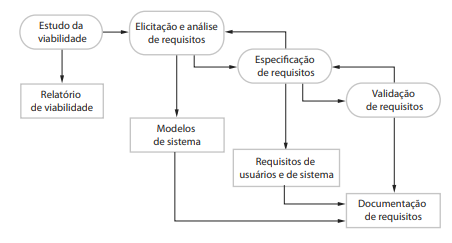
\includegraphics[width=0.6\textwidth]{img/eng_req.png}
    \caption{Processo de engenharia de requisitos \cite{Sommerville07}}
    \label{fig:eng_req}
\end{figure}


De acordo com Sommerville \cite{Sommerville07}, as atividades decorrentes do processo não são realizadas de forma linear e sequencial. Até alcançar a fase de entrega final, várias iterações novas são pensadas para novas definições, especificações e revisões dos requisitos, mostrando que tais etapas são de certa forma ligadas em cadeia. Nos modelos ágeis de desenvolvimento, como o \textit{Extreme Programming}, os requisitos são criados, desenvolvidos e entregues de forma a incrementar sempre a iteração anterior de acordo as necessidades básicas e essenciais do usuário, enquanto o processo de elicitação de requisitos é feita pelos usuários que estão testando a ferramenta juntamente com o time de desenvolvedores.
 
 Segundo Fleming \cite{cmmi}, a área de engenharia de requisitos tem em mente três pontos em específico: 
 
 \begin{enumerate}
     \item A área de desenvolvimento de requisitos do cliente fornece um conjunto de requisitos por parte do usuário que vão fornecer os requisitos para o desenvolvimento dos requisitos do produto;
     \item A área de desenvolvimento de requisitos de produto fornece a partir dos requisitos dos componentes do produto o design a ser usado nos produtos ou em seus componentes;
     \item A análise e a validação dos requisitos fornece a necessidade de análise do usuário, produto e dos componentes do produto para definir, extrair e entender os requerimentos.
 \end{enumerate}

 As práticas do terceiro ponto, em específico, levam a suportar as práticas em especificações nos dois primeiros pontos em específico. O processo associado com a área de engenharia de requisitos e correlatas podem servir integralmente para a área técnica responsável, a qual pode interagir de forma recursiva, contribuindo também na agilidade do desenvolvimento do produto para o usuário final.
 
 \subsection{Elicitação de Requisitos}
 
 Uma das primeiras atividades a serem realizadas nos processos de Engenharia de Requisitos (\acrshort{ER}) é a elicitação de requisitos, onde esta se passa pelos processos de aprendizado, imersão e descoberta de necessidades \cite{Hadar}. Esta área está diretamente ligada as origens dos requisitos do sistema e como os responsáveis pela engenharia de software conseguem coletá-los \cite{SWEBOK2014}. Para tanto, os profissionais da área, junto aos clientes e usuários finais do sistema em criação, trabalham de forma a obter insumos e dados a respeito o domínio da aplicação, os serviços a serem ofertados pelo sistema, como ele se desempenha, quais as limitações de hardware e assim por diante, de acordo Sommerville \cite{Sommerville07}.

Essa atividade é realizada de forma puramente humana, onde os \textit{stakeholders} são identificados e, a partir daí, o relacionamento entre equipe de desenvolvimento e cliente são consolidadas \cite{SWEBOK2014}. Essa atividade passa pelo envolvimento de diversos tipos de perfis dentro de uma organização, como por exemplo os próprios \textit{stakeholders}, onde também se inserem os usuários finais que irão usar o sistema e/ou qualquer outra pessoa que seja afetada com este uso, de acordo Sommerville \cite{Sommerville07}.

A elicitação tem como foco a identificação do problema, proposição de elementos para a solução, a negociação de abordagens distintas e a especificação de um conjunto primitivo de requisitos do produto em um ambiente que seja apto para o alcance deste objetivo \cite{pressman}. Um dos aspectos principais para uma elicitação de requisitos ser alcançado com sucesso é a fácil e eficiente comunicação entre os diversos \textit{stakeholders} \cite{SWEBOK2014}.

Para tanto, é necessário uma coleção de modelos que seja consistente nos mais variados níveis de abstração, visando facilitar a comunicação entre os usuários do sistema (\textit{stakeholders}) e os engenheiros de software \cite{SWEBOK2014}. Temos a disposição vários tipos de modelos de elicitação e análise de requisitos, onde para cada organização temos a sua versão ou instância que dependem de fatores ambientais locais, como por exemplo o nível de conhecimento do pessoal, a espécie de sistema a ser criado, quais normas serão usadas, entre outros \cite{Sommerville07}. 
 
\section{Desenvolvimento Ágil de Software}

Idealizado em 2001 em uma carta pública divulgada na internet, o manifesto ágil, criado por Kent et al. \cite{agilemanifesto} veio para se transformar em uma revolução na forma de transformar os projetos para criação de produtos baseados em programação. Com o lema de valorizar indivíduos e interações, software em funcionamento, colaboração com o cliente e responder as mudanças, a mudança de paradigma que o manifesto trouxe na produção de software foi imediata, sendo estes princípios derivados a partir do modelo \textit{Extreme Programming}, também conhecido como \acrshort{XP}. Com este modelo de desenvolvimento, o foco deixa de ser um modelo de construção de software em cascata, sem interações e respostas rápidas para um modelo muito mais adaptável e maleável de acordo as necessidades de negócio. Para Sommerville \cite{Sommerville07}, tais características do desenvolvimento ágil de software se passava pelos seguintes princípios:

\begin{itemize}
    \item \textbf{Envolvimento do cliente}: O cliente precisa estar a par do que se sucede durante o desenvolvimento de seu produto, sempre fazendo uma constante verificação da criação e resultado de seu sistema além de poder sugerir implementações e melhorias durante este processo.
    
    \item \textbf{Entrega incremental}: O desenvolvimento do produto é feito de forma incremental e individual junto ao cliente.
    
    \item \textbf{Pessoas, não processos}: As equipes devem ter suas habilidades de desenvolvimento do produto reconhecidas e permitindo seu desenvolvimento com liberdade, permitindo assim que os membros possuam suas peculiaridades respeitadas e sem manuais pré-definidos.
    
    \item \textbf{Aceitar as mudanças}: É necessário ter em foco que os requisitos do sistema irão mudar com o tempo de desenvolvimento, por isso o sistema deve ser desenvolvido permitindo a alteração e acomodação destas alterações não previstas.
    
    \item \textbf{Manter a simplicidade}: Manter sempre em vista o lado simples das coisas, seja do software a ser criado quanto dos processos de desenvolvimento deste programa, trabalhando de forma proativa para eliminar possíveis complexidades que o sistema possa a vir a apresentar quando possível.

\end{itemize}

\subsection{Metodologia Scrum}

Scrum é uma metodologia ágil para gestão e planejamento de projetos de software. Um framework dentro do qual pessoas podem tratar e resolver problemas complexos e adaptativos \cite{desenvolvimentoagil}. De acordo Schwaber e Sutherland \cite{Scrum}, mesmo sendo uma metodologia fácil de entender e de baixo recursos, é um método de difícil execução, por ser difícil de dominar. Segundo Pressman \cite{pressman}, o entendimento e forma de lidar do Scrum batem diretamente com o manifesto ágil. A metodologia Scrum é formada por times, papéis, eventos, artefatos e regras, conforme apresentando na Tabela \ref{table:1}.

Cada um dos elementos nesta metodologia tem um foco específico e são cruciais para sucesso no uso. Schwaber e Sutherland \cite{Scrum} descrevem os principais pilares que são utilizados pela metodologia Scrum: Transparência; Inspeção; Adaptação. De acordo os membros do times aprendem e exploram os valores supracitados conforme lidam com os projetos usando a metodologia, percebe-se que os valores de comprometimento, coragem, foco, transparência e respeito são abraçados e se tornam parte comum no time. Conforme estes valores são internalizados há mais vivência com eles, as chances de sucesso no uso da metodologia \cite{Scrum}.

\begin{table}[h!]
    \centering
    \caption{Time, artefatos e eventos do \textit{Scrum} \cite{Scrum}}
    \small
    \begin{tabular}{|p{3cm}|p{12cm}|}
        \hline
        \textbf{Papel} & \textbf{Descrição}\\ 
        \hline
        \textit{Product Owner} & Profissional responsável por entregar o máximo possível de valor do time de desenvolvimento e do produto.\\
        \hline
        Time de Desenvolvimento & Equipe de técnicos responsáveis pela entrega de uma versão utilizável do produto a cada \textit{Sprint}.\\
        \hline
        \textit{Scrum Master} & Profissional responsável pela fixação da teoria, práticas e regras do \textit{Scrum} e garantir que esta metodologia esteja em conformidade. \\
        \hline
        \textbf{Artefato} & \textbf{Descrição}\\  
        \hline
        \textit{Backlog} do Produto & Descrição de tudo o que o produto deve ter, estando este em constante evolução e sempre fornecendo de referência para as mudanças a serem registradas no produto.\\ 
        \hline
        \textit{Backlog} da \textit{Sprint} & É composta pelos itens da Product Backlog selecionados para aquela \textit{Sprint}, mais o plano de como entregar o incremento do produto e atingir os objetivos da \textit{Sprint}. Os itens são analisados pela equipe de desenvolvimento e divididos em tarefas. \\
        \hline
        \textbf{Evento} & \textbf{Descrição}\\
        \hline
        \textit{Sprint} & Parte central do \textit{Scrum} que ocorre por um tempo de duas a quatro semanas, período onde uma parte do produto é criada.\\
        \hline
        Reunião de Planejamento de \textit{Sprint} & Evento onde trabalho a ser realizado na \textit{Sprint} é planejado na por todo o Time Scrum. \\
        \hline
        Reunião Diária & Reunião com duração máxima de 15 minutos, para que o Time de Desenvolvimento possa informar o que foi realizado de trabalho no dia anterior, o planejamento do dia corrente e os possíveis bloqueios que estejam ocorrendo para o progresso da \textit{Sprint}.\\
        \hline
        Revisão da \textit{Sprint} & Reunião realizada ao final da \textit{Sprint} para revisar o incremento e adaptar o Backlog do Produto se necessário.\\
        \hline
        Retrospectiva da \textit{Sprint} & É uma oportunidade para o Time Scrum inspecionar a si próprio e criar um plano para melhorias a serem aplicadas na próxima Sprint.\\ 
        \hline
    \end{tabular}
    \label{table:1}
  \end{table}

No Scrum, as funcionalidades a serem implementadas em um projeto são mantidas no Backlog do Produto. O processo de desenvolvimento ocorre de forma iterativa, e cada iteração se dá o nome de \textit{Sprint}. as quais possuem um prazo de duas a quatro semanas para a sua conclusão. A cada \textit{Sprint}, se realiza uma Reunião de Planejamento de \textit{Sprint}, um evento onde o Product Owner prioriza os itens do Backlog do Produto e a Equipe de Desenvolvimento separa as atividades que ela será capaz de implementar durante a \textit{Sprint} que se inicia. As atividades selecionadas para a \textit{Sprint} são enviadas do Backlog do Produto para o Backlog da \textit{Sprint}. Além disso, a cada dia, a Equipe de Desenvolvimento faz reunião de breve duração (geralmente até 15 minutos) com o foco em alinhar o conhecimento dos membros da equipe sobre o trabalho que está sendo desenvolvido, além do planejamento para o dia e possíveis bloqueios que possam estar se sucedendo durante a execução dos trabalhos. Ao final de uma \textit{Sprint}, a equipe realiza uma Revisão da \textit{Sprint}, onde são mostrados as funcionalidades implementadas ou o que pode ter falho durante a entrega. No fim, é realizada uma Retrospectiva da \textit{Sprint} onde a equipe avalia o que foi realizado, o que faltou realizar e faz o planejamento da futura \textit{Sprint} \cite{Scrum}.

\begin{figure}[h!]
    \centering
    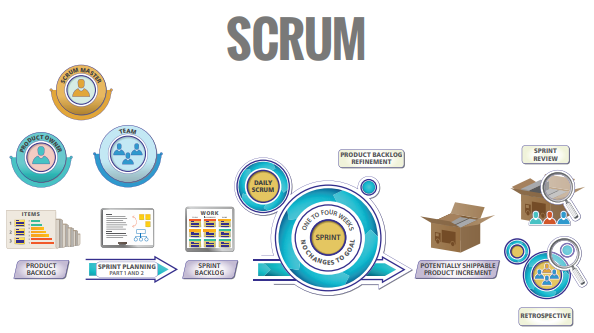
\includegraphics[width=0.6\textwidth]{img/Imagem Scrum Primer.png}
    \caption{Como uma Scrum é planejada, executada e seus membros \cite{primer}.}
    \label{fig:scrum}
\end{figure}

\subsection{Planning Poker}

O Planning Poker consiste em uma técnica de estimativa lúdica e de fácil execução voltada a metodologias ágeis, com o foco em tamanho de complexidade da estória para todos os membros de um time ágil \cite{planningpoker,usingfunctionpoints,storyestimation}. Este modelo é voltado para que cada membro possa colocar em vista durante a reunião de planejamento do projeto a ser executado como aquela história \cite{Scrum}. Durante este processo, a equipe de desenvolvimento e os especialistas do negócio (geralmente o Product Owner) juntamente com um Scrum Master, se juntam para chegarem em um consenso coletivo relacionado às complexidades dos trabalhos a serem executados \cite{techplanningpoker}. Geralmente, este processo tende a criar resultados mais aceitáveis quanto ao menor risco e menos erros nas estimativas \cite{usingplanningpoker2}.

Neste processo, os participantes da reunião são providos de um \textit{deck} de cartas para o Planning Poker. Cada carta possui um valor único, como por exemplo 0, 1/2, 1, 2, 3, 5, 8, 13, 20, 40 e 100 e ``?", geralmente utilizado quando o membro não sabe estimar o valor e deixa em aberto para a discussão e definição na rodada seguinte. Outra série comumente utilizada é a série de Fibonacci para os valores das cartas. Não se existe um consenso a respeito tais valores, porém geralmente a sequência de Fibonacci é a mais comum a ser utilizada \cite{evaluatingplanningpoker}.

\begin{figure}[h!]
    \centering
    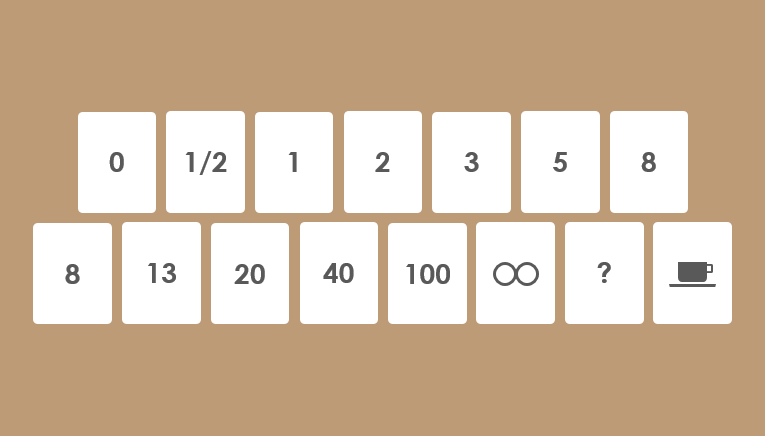
\includegraphics[width=0.6\textwidth]{img/planningpoker.png}
    \caption{Exemplo de cartas de um Planning Poker \cite{visual}.}
    \label{fig:planningpoker}
\end{figure}


Os processos e os passos para o Planning Poker são simples e de fácil aplicação \cite{usingplanningpoker2}. Primeiramente, uma história de usuário será pega pelo moderador do jogo. Depois, o representante do cliente ou o Product Owner explica de forma clara, visando que todos os envolvidos entendam a história com atenção. Em caso de qualquer questão, o Product Owner é o responsável pela resposta. Logo após, cada participante estima o tamanho da história mostrando a carta que indique um valor. Este valor deve ser selecionado. Este valor deve ser selecionado ao considerar fatores influenciantes, como a complexidade e o risco de negócio envolvendo a história, por exemplo. Caso haja um consenso no valor das cartas apresentadas por todos os membros envolvidos, o valor é dado à história e o time escolhe outra história para a estimativa. Caso contrário, o membro ou os membros do Planning Poker que escolheram o maior e o menor valor precisam explicar os motivos do porquê terem dado aquele valor para a história e defenderem sua sugestão de valor. Após este ponto, o time conversa entre si sobre a história e discute a respeito de suas especificações, requerimentos e limitações em detalhe. Imediatamente após a discussão, a estimativa deve ser reavaliada. Este processo deve ser feito até que o time chegue a um consenso no valor da história. Após o consenso, este passo deve ser repetido para todas as histórias que fazem parte daquela reunião de planejamento e, assim, passarem a fazer parte da \textit{Sprint} corrente. \cite{predictingdevelopment}.

De acordo Gandomani et al. \cite{gandomani}, após um estudo em uma empresa anônima, foi verificado que para o modelo funcionar é necessário maturidade da equipe como um todo, desde o processo de estimativa até o julgamento final entre a equipe para estimar corretamente a complexidade da história, porém nada impede que em algumas horas o time chegue a um consenso sem longas conversas entre si, acreditando no que um dos membros tem a relatar daquela história ou que em determinadas horas as longas conversas sejam necessárias para, assim, se chegar ao consenso final. De acordo o autor, este segundo ponto costuma trazer maior precisão na estimativa da complexidade do projeto. Porém, para ter chego a tal ponto, é necessário que a equipe trabalhe em regime colaborativo para que o consenso venha de forma mais natural e precisa.

\section{Inteligência Artificial}

Quando abordamos o assunto ``inteligência artificial´´, temos uma complicada missão para a definição deste conceito, porém ao longo do tempo este assunto se dividiu entre quatro linhas de raciocínio:

\begin{enumerate}
    \item Sistemas que pensam como seres humanos: ``O novo e interessante esforço para fazer os computadores pensarem... máquinas com mentes, no sentido total e literal”, de acordo Haugeland \cite{haugeland}.
    \item Sistemas que atuam como seres humanos: ``A arte de criar máquinas que executam funções que exigem inteligência quando executadas por pessoas”, de acordo Stalder \cite{stalder}.
    \item Sistemas que pensam racionalmente: ``O estudo das faculdades mentais pelo seu uso de modelos computacionais.”, de acordo Charniak \cite{charniak}.
    \item Sistemas que atuam racionalmente: ``A Inteligência Computacional é o estudo do projeto de agentes inteligentes.”, de acordo com Poole et al. \cite{Poole}.
\end{enumerate}

Geralmente, as linhas de pensamento 1 e 3 apontam para o processo de pensamento e raciocínio, enquanto as 2 e 4 ao comportamento. Além disso, as linhas de pensamento 1 e 2 aferem o sucesso em razão à fidelidade relacionada ao desempenho humano, enquanto na 3 e 4 aferem o sucesso, fazendo uma comparação a um conceito ideal de inteligência, que se chamará de racionalidade. Um sistema é racional, inteligente se ``executa tudo de acordo” com os dados fornecidos a ele, segundo Russel e Norvig \cite{russelnorvig}.

Historicamente, as quatro perspectivas para o estudo da inteligência artificial têm sido seguidas. Sem surpresas, há uma tensão entre abordagens com o foco ao redor seres humanos e abordagens focadas na racionalidade. Uma abordagem focada em seres humanos precisa ser feita com o empirismo, envolvendo hipóteses e afirmação através de experimentos científicos. Enquanto isso, a abordagem racionalista é um misto de matemática e engenharia \cite{russelnorvig}.

A \acrshort{IA} ainda é um assunto de difícil complexidade dependendo do tema atrelado ao qual é abordado. Ainda não sabemos se o homem seria capaz de criar a real inteligência artificial, ou chegar perto de construir um simulacro que possa descobrir as bases de como o cérebro humano se comporta, que é a base sua criação. Hoje, o que temos são que seus conceitos desenvolvidos ao longo de anos trazem incontáveis progressos e benesses para humanidade e que de certa forma ela sempre inovará e evoluirá gradativa e progressivamente \cite{reynoldsstair}.

Segundo Russel e Norvig \cite{russelnorvig}, suas bases encontram-se em distintos campos, a partir de distintas perguntas, perspectivas e desafios, conforme apresentado na Tabela \ref{table:2}.

\begin{table}[h!]
    \centering
    \caption{Relação campo versus pergunta \cite{russelnorvig}}
    \small
    \begin{tabular}{|p{3cm}|p{12cm}|}
        \hline
        Filosofia & Podem ser utilizadas regras formais para tirar conclusões válidas? Como a mente funciona em um cérebro físico? De onde vem o conhecimento? Como o conhecimento leva a ação?\\ 
        \hline
        Matemática & Quais são as regras formais para tirar conclusões válidas? O que pode ser computado? Como raciocinamos com informações incertas?\\
        \hline
        Economia & Como devemos tomar decisões para maximizar o retorno? Como devemos fazer isso quando outros não podem ir junto? Como devemos fazer isso quando a recompensa pode estar longe no futuro?\\
        \hline
        Neurociência & Como os cérebros processam informações?\\
        \hline
        Psicologia & Como os seres humanos e os animais pensam e agem?\\
        \hline
        Engenharia e Computação & Como podemos construir um computador eficiente??\\
        \hline
        Teorias de Controle e Cibernética & Como as maquinas podem operar sob seu próprio controle?\\
        \hline
        Linguística & Como a linguagem se relaciona com o pensamento? \\
        \hline
    \end{tabular}
    \label{table:2}
\end{table}

De forma geral, para Kaufman \cite{kaufman} e em um olhar simplificado, podemos pensar a \acrshort{IA} como uma reexecução dos comportamentos que o cérebro humano pode controlar. A ação de dançar, por exemplo, é controlada pelo cérebro (acompanhar o par, coordenação da movimentação no ritmo de partes do corpo em geral), assim como o respirar é igualmente controlado pelo cérebro, mesmo que de forma indireta: as sensações que chegam no cérebro são parte do domínio da inteligência, estando potencialmente no campo da \acrshort{IA}. Porém, o ``processo mental'' da \acrshort{IA} supera o processo mental humano, se, por um lado, a \acrshort{IA} executa tarefas que são por suposto competências dos seres humanos, sua capacidade ultrapassa limitações humanas como observado em distintas situações do dia a dia com o uso das tecnologias apropriadas, como por exemplo, um jogo de xadrez \cite{xadrez} ou Go \cite{gojogo}. 

\section{Ética em IA}

A palavra ética, tentando simplificar uma coisa que de forma alguma pode ser chamada de simples, indica um tipo de comportamento adquirido ou conquistado, portanto, não-instintivo. Trata-se, de toda forma, um modo de um ser humano, construído socialmente com base nas relações entre os seres humanos na sociedade. Refere-se diretamente a natureza da ação humana. Se a IA representa uma nova espécie inteligente coexistindo com a espécie humana, nos parece legítimo supor que precisamos de uma nova ética. Este nos parece um dos maiores desafios posto no campo das ciências sociais, envolvendo a revisão de conceitos tradicionais e a elaboração de novos que permitam lidar com a complexidade decorrente dessa convivência entre duas espécies inteligentes, com a perspectiva de num futuro relativamente breve existir a dominância de uma sobre a outra (IA sobre os humanos)\cite{kaufman}.

Para Kaufman \cite{kaufman}, dentro das questões que são consequência dos recentes avanços, a autonomia dos sistemas inteligentes se caracteriza como uma das mais relevantes, e não em vão uma das mais difíceis pela sua própria natureza: autonomia é uma prerrogativa inerente ao processo de aprendizado das máquinas (\textit{Deep Learning}).

Dois dos conceitos que são referidos na literatura são: responsabilidade social e ética. A literatura apresenta diversos pontos de vista sobre estes conceitos. Para Fischer \cite{socialresponsability}, responsabilidade social e a ética são conceitos muitas das vezes utilizados de maneira indiferenciada. Por exemplo, a responsabilidade social é posta como sendo a ética em um determinado contexto organizacional; a responsabilidade social empenha no impacto que a atividade do negócio tem em toda a sociedade. Enquanto que o conceito de ética está relacionado com a conduta daqueles que fazem parte da organização. A literatura não apresenta relação entre a responsabilidade social e a ética, apresentando ainda que a responsabilidade social tem diversas dimensões, entre elas a ética \cite{socialresponsability}. Um terceiro conceito revisto na literatura é a moralidade. De acordo com Beauchamp e Bowie \cite{ethicaltheory}, a moralidade refere-se a princípios ou regras de conduta moral tal como estão definidas na sociedade. A moralidade existe antes da aceitação ou rejeição dos seus standards pelos indivíduos, nesse sentido a moralidade não pode ser meramente uma política ou um código. Nesse sentido, a ética tem a ver com o refletir sobre a natureza e justificações do certo e do errado \cite{ethicaltheory}.

Os sistemas baseados em \acrshort{IA}, de acordo com Guizzardi et al. \cite{guizzardi2020ethical} não são agentes morais que podem agir com uma razão com base em princípios éticos. Pelo contrário, são softwares que tem suas funcionalidades e qualidades baseadas em requerimentos éticos, em adição a outros tipos de requerimentos que são requisitados para o preenchimento.

Existe na literatura uma profusão de artigos que investigam como os sistemas baseados em IA devem ser agentes morais que tomam decisões éticas em tempo de execução \cite{guizzardi2020ethical}, por exemplo um carro decidir entre atropelar uma ou mais pessoas, um software não desligar a luz por situação social ou soltar poluentes em um navio não-tripulado em uma área de preservação que mate corais ou peixes em alto-mar. Em contrapartida, estamos interessados em investigar como elicitar requisitos éticos para sistemas baseados em IA para que eles estejam em conformidade com diretrizes e princípios éticos e outras funcionalidades que devam ter \cite{guizzardi2020ethical}.
 
\subsection{Princípios}

Múltiplos princípios éticos foram apresentados por diversas instituições publicas, privadas, não governamentais e instituições de ensino. Nestes documentos, os termos princípios e diretrizes às vezes aparecem de formas intercambiáveis, ao longo deste trabalho assumimos que as diretrizes de ética em IA são um conjunto de princípios éticos. Ou seja, as diretrizes de ética em IA possuem princípios. As principais diretrizes de ética em IA mais reconhecidas pela comunidade são \acrshort{AI HLEG}\cite{HLEG_EthicsGuidelinesForTrustworthyAI} e \acrshort{IEEE} \acrshort{EAD}v1 \cite{ieee2020EADv1}.

Diversos estudos tiveram com objetivo a compilação de princípios éticos presentes na literatura em um único conjunto \cite{hagendorff2020ethics}, \cite{jobin2019global}, \cite{Fjeld2020principled}, \cite{Zeng2019LinkingAI}, \cite{koensmit2020areviewofaiprinciples}. Um desses estudos, o qual nos auxiliou a direcionar tais princípios para a implantação de ética em \acrshort{IA}, foi elaborado por Ryan e Stahl \cite{Ryan2020ArtificialIE}. Neste trabalho, os autores buscaram por princípios éticos que possam auxiliar desenvolvedores e usuários na implementação e entendimento de ética em IA. Esta compilação feita em 11 princípios é apresentada brevemente na tabela abaixo:

\begin{footnotesize}
\begin{longtable}
{|l|p{3.6cm}|p{10.5cm}|}
\caption{Princípios e suas questões éticas apresentadas no trabalho de Ryan e Stahl \cite{Ryan2020ArtificialIE}}
 \label{tab:ryanstahlprincipios}
\\ \hline
\# & Princípio & Questões éticas
\\ \hline

1 & Transparência & Explainabilidade; Explicabilidade; Compreensibilidade; Interpretabilidade; Comunicação; Divulgação; Apresentação
\\ \hline

2 & Justiça e equidade (\textit{fairness}) & Consistência; inclusão; igualdade; equidade; não-viés; não-discriminação; diversidade; pluralidade; acessibilidade; reversibilidade; remediar; reparação; contestação; acesso; distribuição
\\ \hline

3 & Não-maleficência & Segurança; proteção / \textit{safety}; dano; precaução; prevenção; integridade; não-subversão
\\ \hline

4 & Responsabilidade & Responsabilização / \textit{accountability}; responsabilidade / \textit{liability}; agir com integridade
\\ \hline

5 & Privacidade & Informação pessoal ou privada
\\ \hline

6 & Beneficência & Bem-estar; paz; bem social; bem comum
\\ \hline

7 & Liberdade e autonomia & Consentimento; escolha; auto-determinação; liberdade / \textit{liberty}; empoderamento
\\ \hline

8 & Confiança & Confiabilidade / \textit{Trustworthiness}
\\ \hline

9 & Sustentabilidade & Meio ambiente (natureza); energia; recursos (energia)
\\ \hline

10 & Dignidade & Dignidade
\\ \hline

11 & Solidariedade & Segurança social; coesão
\\ \hline
\end{longtable}
\end{footnotesize}

Neste trabalho iremos utilizar como prova de conceito os princípios baseados no sistema ECCOLA \cite{ECCOLA}, o qual também tem como fundamentações as práticas pregadas pelo \acrshort{IEEE} \acrshort{EAD}v1 \cite{ieee2020EADv1} e pelo \acrshort{AI HLEG}\cite{HLEG_EthicsGuidelinesForTrustworthyAI}.


\section{Trabalhos relacionados}

Foram encontradas na literatura um conjunto de ferramentas que auxiliam a implementação de ética em IA \cite{siqueira2021ethical}. Neste estudo foi explorado um repositório de código aberto GitHub onde foram encontradas 21 ferramentas disponíveis publicamente que auxiliam a implementação de ética em IA, porem apos o sistema ter sido desenvolvido, e com grande foco no principio de Explicabilidade. 

Outro estudo \cite{morley2019initial} encontrou 106 ferramentas, estas porém, em geral, necessitam de adaptação para o contexto do desenvolvedor, ou seja, não são software de prateleira (\textit{off-the-shelf}), focam em partes especificas do processo de desenvolvimento de software. Tais ferramentas dispões de falta de documentação e usabilidade, além necessitarem uma forte alteração para se adequarem ao ambiente as quais deverão ser usadas.

O que mais se assemelha a proposta do nosso trabalho é o do Vakkuri et al. \cite{ECCOLA}, onde um baralho de cartas é utilizado para auxiliar times de desenvolvimento a elicitar requisitos éticos em IA no contexto de desenvolvimento ágil. Portanto, nossa proposta envolverá a implementação deste método, ECCOLA, como uma Prova de Conceito.

\section{Síntese do Capítulo}

Vimos neste Capítulo a síntese teórica dos tópicos aos quais abordaremos na construção do guia de ética para aplicações no contexto de \acrshort{IA}. Demos uma passa desde as origens da engenharia de software, como ela formou a necessidade de formalizações para as definições em um projeto para a criação de um software, no qual resultou a engenharia de requisitos, área a qual auxilia a entender e levantar os requisitos necessários para o software atendendo aos desejos de seu solicitante. Com isso, vimos como o processo de elicitação de requisitos se forma em uma importante área para a correta avaliação de acordo seu \textit{stakeholder}. Foi verificado também como o desenvolvimento ágil de software nasceu visando que tais softwares não fossem criados apenas de forma rápida, porém também otimizando os recursos de tempo e dinheiro gastos durante a sua criação, e vemos como o Scrum é um dos métodos mais populares, onde em determinada fase do uso desta metodologia (a fase de planejamento da sprint), temos o uso de um jogo de cartas que, de forma divertida e de fácil entendimento, ajuda aos desenvolvedores avaliar o nível de complexidade de cada história a ser trabalhada em cima. Foi visto também os conceitos de inteligência artificial e quais são as suas implicações éticas, áreas em que o debate é essencial durante a fase de planejamento. Para o Capítulo \ref{desenvolvimento}, será apresentado o desenvolvimento de um guia em forma de \textit{Planning Poker} para auxiliar no debate de quais questões éticas que a \acrshort{IA} a ser desenvolvida deverá se fundamentar, atendendo ao escopo e necessidades de seus \textit{stakeholders}.











